%
% File: chap_3.tex
% Author: Yuil Tripathee
%
\chapter{Requirements Elicitation}

\section{Elicitation Techniques}

\textit{TODO: Before analyzing the system, various technique are employed to gather its requirements.}

\textit{TODO: Explain:}

\begin{itemize}
	\item Interviews
	\item Questionnaires
	\item Workshops
	\item Observation
	\item Prototyping
\end{itemize}

\section{Stakeholders}

\section{System Analysis - Data Flow}

\textit{TODO: Data Flow diagram}

\section{Use Case Analysis}

\begin{figure}[!h]
	\centering
	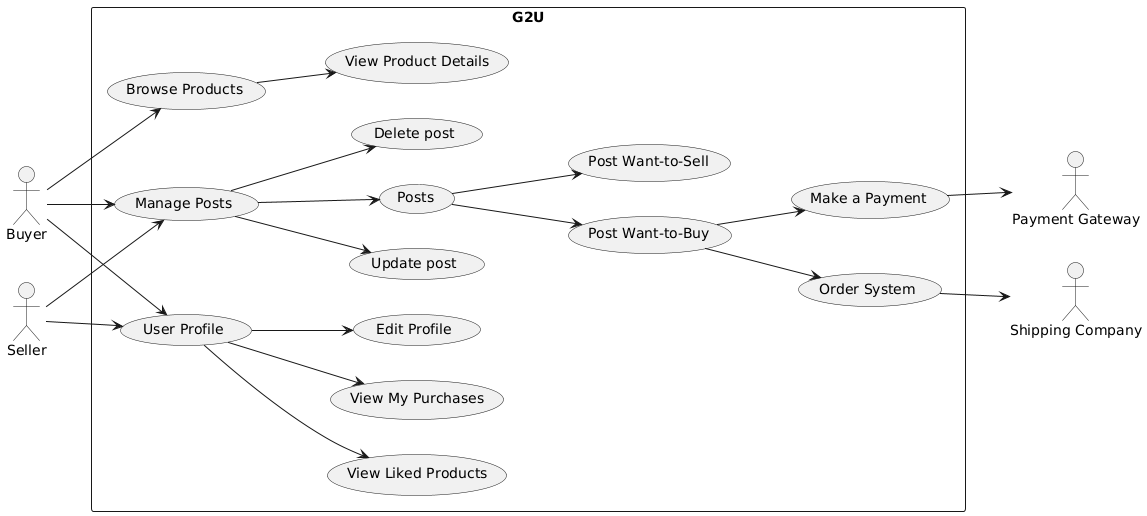
\includegraphics[width=1\textwidth]{chapters/ch-03/00_usecase.png} % Adjust width as needed
	\caption{Latest version of use case diagram after feedback driven iteration}
	\label{fig:usecase} % Label for referencing the figure
\end{figure}

For software engineering observers, it is evident that use case diagram (in the Figure ~\ref{fig:usecase}) presented here is not in line with the data flow diagram. This is the result of agile practice. We kept data flow analysis out of SDLC loop as it is redundant to sequence diagram (below). We can effectively model both system behavior, reaction (in terms of data changes and transfers) much effectively across our implementation team.

\section{Functional Design}

\textit{TODO: Here are some functional requirements (example)}

\begin{itemize}
	\item User Registration
	\item Tutor Scheduling and Availability
	\item Online class
\end{itemize}

\textit{TODO: Translate this to user story when doing Kanban}

\textit{TODO: Each functional requirements should have details and implementation in description list}

\section{Other Non-functional requirements}

\textit{TODO: Quantize these requirements}

\begin{itemize}
	\item Scalability
	\item System Availability
	\item Security
	\item Usability
	\item Performance
\end{itemize}

\subsection{Mandated constraints}

Examples include: Economics

\subsection{Regulatory compliance}

\clearpage